When visualizing the ligand trajectory in its original form, e.g., using a line strip of consecutive ligand positions, the visualization becomes very crowded even when analyzing only few hundreds of snapshots (see Figure~\ref{fig:crowded} left).
Therefore, it is necessary to simplify the original trajectory data and to visualize this simplified version.
In this manner, we enable the user to deduce the information about significant ligand movements directly from its 3D visualization.

\begin{figure}
	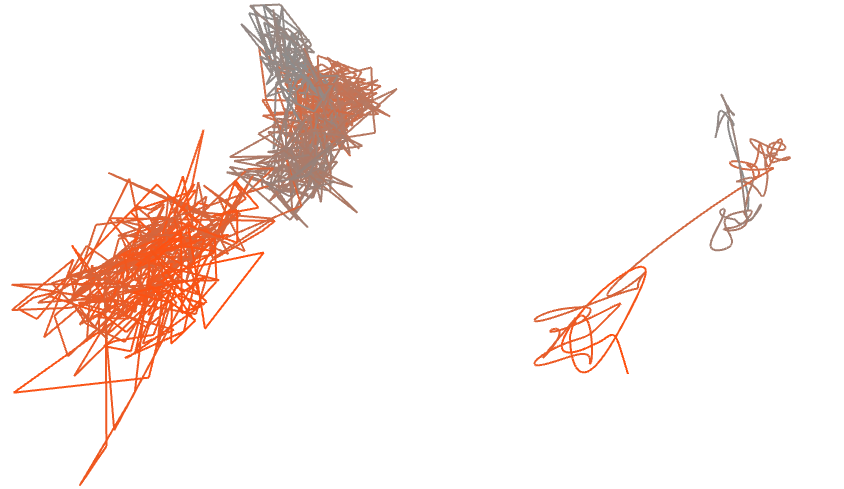
\includegraphics[width=0.95\linewidth]{img/crowded-combined.png}
\caption{Visualization of 800 snapshots of a ligand trajectory using line strip.
Visualization of the original trajectory is crowded (left).
On the other hand, visualization of the simplified trajectory clearly reveals its possible important parts (right).
The trajectory is colored by time from beginning (gray) towards its end (orange).}
\label{fig:crowded}
\end{figure}

We propose two types of ligand trajectory simplification: i) automatic and ii) interactive.
The automatic simplification is applied to the whole original trajectory, while the interactive one enables fine user-regulated control over the level of simplification of individual parts of the trajectory.
%In fact, the automatic simplification can be viewed as an iterative application of the manual simplification.
%, since its design was aligned with the workflow of a biochemist. - dala by som prec, postradam logicku navaznost
\subsubsection*{Interactive Simplification}

First, we will describe the algorithm for the interactive trajectory simplification (see Algorithm~\ref{alg:simplify}).
The input of the algorithm consist of trajectory $T_{in}$ and interval $I$ which denotes a part where the trajectory should be simplified.
%a data structure describing the simplification ($S$).
%More precisely, $S$ is a list of consecutive intervals that span the whole trajectory.
%Each interval in $S$ is assigned with a simplification level and as such describes amount of simplification of a respective part of $T_{in}$.
%This representation enables simplification of different parts of $T_{in}$ using different level of detail.
As a first step, the algorithm retrieves from a cache the current visualized trajectory $T'$ together with its simplification $S'$.
Structure $S'$ is a list of consecutive intervals that span the whole trajectory.
Each interval in $S'$ is assigned with a simplification level and as such describes the amount of simplification of a respective part of $T_{in}$.
This representation enables the simplification of different parts of $T_{in}$ using different levels of detail.
In the next step, the updated simplification $S$ is obtained by applying $I$ to $S'$.
Then, it is decided whether $T'$ can be incrementally updated to obtain $T_{out}$.
%If so, an interval $\Delta I$ which updates $S'$ to $S$ is obtained and the current visualized trajectory $T'$ is simplified on $\Delta I$ resulting in $T_{out}$.
This is true when the level of simplification of $T'$ at the updated interval $I$ is lower than the desired level of simplification.
In this case, the current visualized trajectory $T'$ is simplified on $I$ resulting in $T_{out}$.
%a difference of $S$ and $S'$ results in a single interval
Otherwise, the visualized trajectory $T'$ cannot be used and the simplified trajectory has to be computed from scratch using $T_{in}$.
This case typically emerges when the user decides to lower the amount of simplification of some part of the trajectory.
The computation then proceeds as follows.
A list $\mathcal{L}$ is computed from $S$.
For each simplification level in $S$, we extract from $S$ a set of all intervals on that level, $L$, and we add $L$ to $\mathcal{L}$.
Then, we iterate through $\mathcal{L}$ in an ascending order by level of simplification.
In each iteration, we have a set of intervals $L \in \mathcal{L}$ and we apply the simplification on all $I_L \in L$ to $T_{out}$.
In both cases, we employ Savitzky-Golay smoothing method~\cite{savitzky1964smoothing} to simplify the trajectory.
As the last step we store the simplified trajectory to a cache.
The caching is employed to primarily improve the performance of automatic simplification.
Moreover, the performance of interactive simplification is also enhanced, for example, when the user iteratively simplifies the same part of the trajectory until reaching satisfiable results.

\begin{algorithm}
  \begin{algorithmic}[1]
	  \Require $T_{in}$ --- trajectory, $I$ --- simplification interval
	  \Ensure $T_{out}$ --- simplified trajectory
		\Procedure{Simplify}{$T_{in}, I$}
			\State $(T', S') \gets$ \Call{CacheLoad}{$ $} \Comment{$S'$ --- previous simplification}
			\State $S \gets$ \Call{Update}{$S', I$}
			\State
			\If{\Call{IsIncremental}{$S, S'$}}
			  %\State $\Delta I \gets$ \Call{Diff}{$S, S'$}
				\State $T_{out} \gets$ \Call{SavitzkyGolay}{$T', I$}
			\Else %\Comment{compute from scratch}
			  \State $\mathcal{L} \gets$ \Call{ByLevels}{$S$} \Comment{$\mathcal{L}$ --- sets of complex intervals}
				\State $T_{out} \gets T_{in}$
				\ForAll{$L \in \mathcal{L}$} \Comment{in asc. order by $level(L)$}
				  \ForAll{$I_L \in L$}
					  \State $T_{out} \gets$ \Call{SavitzkyGolay}{$T_{out}, I_L$}
					\EndFor
				\EndFor
			\EndIf
			\State
			\State \Call{CacheSave}{$T_{out}, S$}
			\State \Return $T_{out}$
		\EndProcedure
  \end{algorithmic}
	\caption{Trajectory simplification}
  \label{alg:simplify}
\end{algorithm}

\subsubsection*{Automatic Simplification}

The automatic algorithm (see Algorithm~\ref{alg:auto-simplify}) is iterative and in its iterations employs Algorithm~\ref{alg:simplify}.
Furthermore, it is based on an idea to simplify only parts of the trajectory that are still too complex.
The algorithm starts with considering the whole trajectory as complex -- the set of complex intervals $C$ is set to the interval spanning $T_{in}$.
Then, the complexity $c$ of $T_{in}$ is evaluated in all points of $T_{in}$.
The complexity $c(x)$ in point $x$ is defined as (see Figure~\ref{fig:complexity}):
\begin{equation}
  c(x) = \sum_{(u, v) \in N(T, x, \nu)}{(|u| + |v|)^2 \alpha(\vec{u}, \vec{v})}, % \mathrm{acos}(\frac{u \cdot v}{|u| \cdot |v|})
\label{eq:complexity}
\end{equation}
where $N(T, x, \nu)$ is a set of consecutive tuples of segments of a trajectory $T$ lying in the neighborhood of $x$ and $\alpha(u, v)$ is an angle between directions of $u$ and $v$.
The neighborhood of $x$ contains all points $y \in T$ such that $d(x, y) < \nu$ where $d(x, y)$ is the distance along $T$.
We evaluate the complexity of $T$ in the neighborhood of $x$ in order to take into account the local shape of the trajectory in the vicinity of $x$.
Our typical setting for $\nu$ is 2~\angstrom\ which is an experimentally obtained value.

\begin{algorithm} [htb]
  \begin{algorithmic}[1]
	  \Require $T_{in}$ --- trajectory, $\nu$ --- complexity neighborhood, $\tau$ --- complexity threshold, $\epsilon$ --- improvement threshold
	  \Ensure $T_{out}$ --- simplified trajectory
		\Procedure{AutoSimplify}{$T_{in}, \nu, \tau, \epsilon$}
			\State $C \gets$ \Call{Interval}{$T_{in}$} \Comment{$C$ --- complex intervals}
			\State $c(x) \gets$ \Call{Complexity}{$T_{in}, \nu$}
			\State
			%\State $S \gets$ \Call{Empty}{$T_{in}$} \Comment{$S$ --- simplification}
			\State $T_{out} \gets T_{in}$
			\Repeat
			  \State $P \gets$ \Call{FindSimplePoints}{$c, \tau$}
				\State $C \gets$ \Call{RemoveSimplePoints}{$C, P$}
			  \State
			  \ForAll{$I \in C$} %\Comment{$I$ --- complex interval}
					\State $T_{out} \gets$ \Call{Simplify}{$T_{out}, I$}
			  \EndFor
				\State
				\State $c'(x) \gets c(x)$ %\Comment{$c'(x)$ --- previous complexity}
				\State $c(x) \gets$ \Call{Complexity}{$T_{out}, \nu$}
				\State
				\State $\Delta c \gets \sum_{x \in T_{out}}{max(c(x) - c'(x), 0)}$
				\State \Comment{$\Delta c$ --- improvement}
			\Until{$\Delta c < \epsilon$}
			\State
			\State \Return $T_{out}$
		\EndProcedure
  \end{algorithmic}
	\caption{Automatic trajectory simplification}
  \label{alg:auto-simplify}
\end{algorithm}

\begin{figure}
	%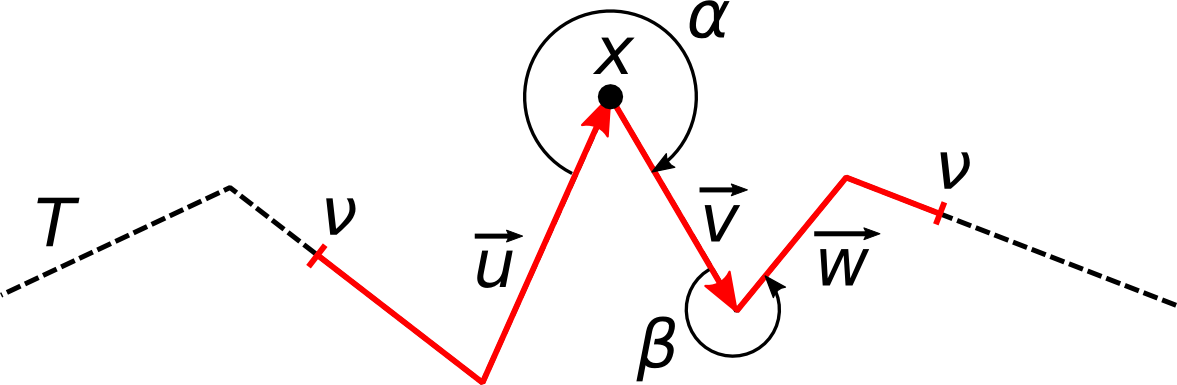
\includegraphics[width=0.95\linewidth]{img/complexity.png}
	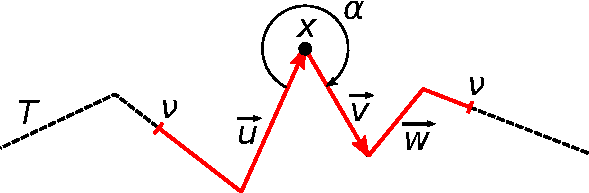
\includegraphics[width=0.95\linewidth]{img/complexity.pdf}
\caption{Evaluation of the complexity of a trajectory $T$ in point $x$.
The complexity $c(x)$ is determined by tuples $(u, v)$ and $(v, w)$, \ie their angles $\alpha$ and $\beta$, as the segments $u$, $v$, and $w$ lie in the neighborhood of $x$ (red).
The neighborhood of $x$ contains all points that are closer (along $T$) to $x$ than to $\nu$.}
\label{fig:complexity}
\end{figure}

Furthermore, the simplification $S$ is set to be empty at the beginning and the resulting trajectory $T_{out}$ is set to $T_{in}$.
The iterative simplification then proceeds as follows.
First, a set of simple points $P$ is found by thresholding $c(x)$ by $\tau$.
All points $p \in P$ are then removed from $C$ which prevents further simplification of parts of the trajectory that are already simple.
Then, $T_{out}$ is simplified in all complex intervals that remained in $C$.
After the simplification, the complexity is evaluated again and the improvement in comparison with the previous complexity is computed.
The iterative simplification ends when the improvement after an iteration $\Delta c$ drops below a user-specified threshold $\epsilon$.

To address the correctness issue, which is raised by trajectory smoothing, we provide the user also with non-smoothing simplification using the Douglas-Peucker algorithm~\cite{visvalingam1990douglas} which preserves original positions.
Generally, the non-smoothing simplification employs schemes presented in Algorithms~\ref{alg:simplify}~and~\ref{alg:auto-simplify}.
Only small modifications to the simplification data structure ($S$) and a new complexity measure $c_{DP}(x)$ were needed due to the nature of the Douglas-Peucker algorithm which keeps only a subset of its input positions.
We present only the new complexity measure since the other changes are trivial.
The complexity $c_{DP}(x)$ is defined as:
\begin{equation}
  c_{DP}(x) = \sum_{s \in N_{DP}(T, x, \nu)}{\frac{|s|}{|P_e - P_s|}},
\label{eq:complexity-dp}
\end{equation}
where $N_{DP}(T, x, \nu)$ is a set of trajectory segments in the neighborhood of $x$ (see Equation~\ref{eq:complexity}), and $P_s$ and $P_e$ are start and end points in that neighborhood.
Both simplification approaches were evaluated by the domain experts.
They concluded that, although the smoothing simplification is superior in the ability to provide results that are easy to understand using visualization, it is important for them to use the non-smoothing simplification to confirm their assumptions that were made using the smoothing variant.